\question DoubleTree hired you to architect one of their hotel expansions!  As
you might expect, their floor plan can be modeled as a tree and the expansion
plan requires doubling each node (the patented double tree floor plan). Here's
what some sample expansions look like:\\\\

\begin{tabular}{c c}
\textbf{Before} & \textbf{After}\\
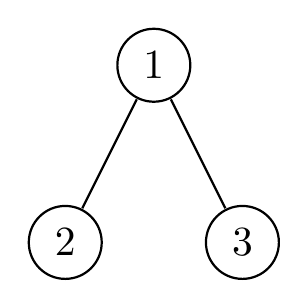
\begin{tikzpicture}[thick, scale=1.5, transform shape]
    \node [circle, draw] (z){$1$}
        child {node [circle, draw] (a) {$2$}}
        child {node [circle, draw] (b) {$3$}}
        ;
\end{tikzpicture}
&
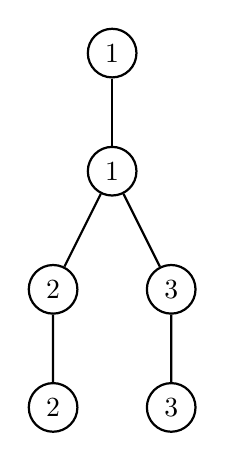
\begin{tikzpicture}[thick, scale=1.0, transform shape]
    \node [circle, draw] (z){$1$}
        child {node [circle, draw] (a) {$1$}
            child {node [circle, draw] (b) {$2$}
                child {node [circle, draw] (d) {$2$}}
            }
            child {node [circle, draw] (c) {$3$}
                child {node [circle, draw] (e) {$3$}}
            }
        }
        ;
\end{tikzpicture}
\end{tabular}

Fill in the implementation for \texttt{double\char`_tree}.

\begin{lstlisting}
def double_tree(t):
    """
    Given a tree, return a new tree where entries appear
    twice.
    >>> double_tree(Tree(1))
    Tree(1, [Tree(1)])
    >>> double_tree(Tree(1, [Tree(2), Tree(3)]))
    Tree(1, [Tree(1, [Tree(2, [Tree(2)]),
                      Tree(3, [Tree(3)])
                     ])
            ])
    """
\end{lstlisting}
\begin{solution}[0.5in]
\begin{lstlisting}
    if t.is_leaf():
        return Tree(t.label, [Tree(t.label)])
    else:
        dbl_branches = [double_tree(c) for c in t.branches]
        return Tree(t.label,
                    [Tree(t.label, dbl_branches)])
\end{lstlisting}
\end{solution}
